\vspace{0.5em}
\subsection{Filtering Stage: $y$-axis and Doppler}

The raw radar point cloud exhibited systematic clutter in the region directly in front of the sensors, primarily due to reflections from the driver's feet and the ground.  
These unwanted detections were consistently observed up to approximately \SI{1.5}{\meter} and persisted even when the vehicle was stationary.  
If left unfiltered, such clutter propagated through the pipeline, degrading clustering and ego-motion estimation.  

To address this, a static filtering stage was implemented with two criteria:
\begin{enumerate}
    \item \textbf{$y$-axis filter:} Only points within the interval $1.5 \leq y \leq 15$~m are retained.  
    This introduces a \textit{dead zone} in front of the vehicle, removing ground clutter and very short-range reflections while keeping the operational range relevant for odometry.
    \item \textbf{Doppler filter:} Only points with radial velocity within $0.01 \leq v_d \leq 8.0$~m/s are accepted.  
    This rejects near-zero Doppler detections (often noise or static artifacts) and unrealistically large outliers.
\end{enumerate}

\noindent
This filtering approach significantly reduced clutter (Fig.~\ref{fig:filter_example}), producing a cleaner point cloud for downstream modules.  
The trade-off is that genuine obstacles appearing within the \SI{1.5}{\meter} dead zone are excluded.  
Although this removes potentially useful information in very close range, the region is dominated by ground clutter and considered less critical for the odometry pipeline.  

\begin{figure}[!htbp]
    \centering
    \begin{subfigure}{0.45\linewidth}
        \centering
        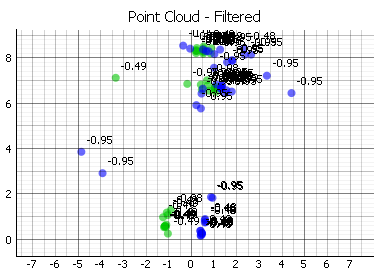
\includegraphics[width=\linewidth]{images/dualSensorClutterYAxis.png}
        \caption{Clutter representation (Radar A = blue, Radar B = green).}
        \label{fig:clutter_representation}
    \end{subfigure}
    \hfill
    \begin{subfigure}{0.45\linewidth}
        \centering
        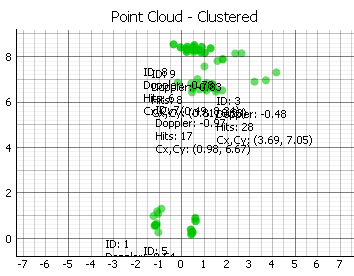
\includegraphics[width=\linewidth]{images/dualSensorClutterYAxisCluster.png}
        \caption{Clustered view of clutter detections.}
        \label{fig:clutter_clustered}
    \end{subfigure}
    \caption{Visualization of unwanted reflections (clutter) near the sensors, dominated by ground and driver-related reflections up to \SI{1.5}{\meter}.  
    Blue dots correspond to Radar A (left), and green dots to Radar B (right).}
    \label{fig:filter_example}
\end{figure}


\FloatBarrier